\section{Special Case: Two Dimensions}\label{sec:special2D}
Consider a two-dimensional feature space where, without loss of generality, feature 1 has a higher weight than feature 2, and agents manipulate their features to move to the nearest point on the (perceived) decision boundary. The agents that will under-invest in the first feature ($\delta_{1_\text{B}}<\delta_{1_\text{NB}}$) will be the ones who satisfy:
 \begin{align}\label{eq:underinvest1}
     \big( \frac{\theta^2}{\norm{\vtheta}_2^2} - \frac{w(\theta)^2}{\norm{\vw(\vtheta)}_2^2} \big)x_1 + \big( \frac{\theta(1-\theta)}{\norm{\vtheta}_2^2} - \frac{w(\theta)(1-w(\theta))}{\norm{\vw(\vtheta)}_2^2} \big)x_2 < \big(\frac{w(\theta)}{\norm{\vw(\vtheta)}_2^2} - \frac{\theta}{\norm{\vtheta}_2^2} \big)\theta_0
 \end{align}
 and the agents who under-invest in the second feature ($\delta_{2_\text{B}}<\delta_{2_\text{NB}}$) will satisfy:
 \begin{align}\label{eq:underinvest2}
     \big( \frac{\theta(1-\theta)}{\norm{\vtheta}_2^2} - \frac{w(\theta)(1-w(\theta))}{\norm{\vw(\vtheta)}_2^2} \big)x_1 + \big( \frac{(1-\theta)^2}{\norm{\vtheta}_2^2} - \frac{(1-w(\theta))^2}{\norm{\vw(\vtheta)}_2^2} \big)x_2 < \big(\frac{1-w(\theta)}{\norm{\vw(\vtheta)}_2^2} - \frac{1-\theta}{\norm{\vtheta}_2^2} \big)\theta_0
 \end{align}
For agents that under-invest in only one of the features, we need one of the \eqref{eq:underinvest1} and \eqref{eq:underinvest2} to be true while the other is not. We rearrange \eqref{eq:underinvest1} and \eqref{eq:underinvest2} to get:
\begin{align}
    \textit{For under-investment in feature 1: }&\alpha x_1 + \beta x_2 < \tau\\
    \textit{For under-investment in feature 2: }&\alpha x_1 + \beta x_2 - (\bar\alpha x_1 + \bar\beta x_2 - \bar\tau) > \tau
\end{align}
Where:
\begin{align}
    &\alpha = \frac{\theta^2}{\norm{\vtheta}_2^2} - \frac{w(\theta)^2}{\norm{\vw(\vtheta)}_2^2}\quad,\quad \beta = \frac{(1-\theta)^2}{\norm{\vtheta}_2^2} - \frac{(1-w(\theta))^2}{\norm{\vw(\vtheta)}_2^2}\quad,\quad \tau = \big(\frac{w(\theta)}{\norm{\vw(\vtheta)}_2^2} - \frac{\theta}{\norm{\vtheta}_2^2} \big)\theta_0 \notag\\
    &\bar\alpha = \frac{\theta}{\norm{\vtheta}_2^2} - \frac{w(\theta)}{\norm{\vw(\vtheta)}_2^2}\quad,\quad \bar\beta = \frac{1-\theta}{\norm{\vtheta}_2^2} - \frac{1-w(\theta)}{\norm{\vw(\vtheta)}_2^2}\quad,\quad \bar\tau = \big(\frac{1}{\norm{\vw(\vtheta)}_2^2} - \frac{1}{\norm{\vtheta}_2^2} \big)\theta_0\notag
\end{align}
By defining $\xi \coloneqq \bar\alpha x_1 + \bar\beta x_2 - \bar\tau$ we can condition on the sign of $\xi$. By using $\xi$ we can say that biased agents:
\begin{enumerate}
    \item Will not under-invest in feature 1 (2) if they under-invest in feature 2 (1) and have $\xi > 0$.
    \item Under-investment (over-investment) in both features is only possible for agents with $\xi < 0$ ($\xi > 0$).
\end{enumerate}
Where:
\begin{align}\label{eq:xi}
    \xi = \big( \frac{\theta}{\norm{\vtheta}_2^2} - \frac{w(\theta)}{\norm{\vw(\vtheta)}_2^2} \big) x_1 + \big( \frac{1-\theta}{\norm{\vtheta}_2^2} - \frac{1-w(\theta)}{\norm{\vw(\vtheta)}_2^2} \big) x_2 - \big( \frac{1}{\norm{\vtheta}_2^2} - \frac{1}{\norm{\vw(\vtheta)}_2^2} \big) \theta_0
\end{align}

Using Proposition~\ref{prop:under-invest-high-dim}, a firm can use $\xi$ as a possible cost or benefit function for their algorithm to, for instance, steer individuals to over-invest in a feature that benefits them more or help them invest less in a feature with a high cost that they have been over-investing in as a result of their bias. After a closer look, \eqref{eq:xi} is the difference between line equations of actual decision boundary and perceived decision boundary.

The following special case illustrates how the agents' behavioral bias will make them under-invest or over-invest in some features in a more straightforward setting:

Consider a setting with two actionable features. We consider a case where $\norm{\vtheta}_2 = \norm{\vw(\vtheta)}_2$. This situation can occur if we look at $\vw(\vtheta)$ as a rotation transform of $\vtheta$. Furthermore, if we consider the function introduced by \cite{Prelec1998}, then for $w(\theta)<\theta$ and in two dimensions, this occurs once for each $\gamma$. This is possible because in two dimensions we can write $\theta>1-\theta$ without loss of generality and by using the function in \cite{Prelec1998} we know that for larger $\theta$ we have $w(\theta)<\theta$. We can write:
\begin{itemize}
    \item Agents that under-invest in feature 1 ($\delta_{1_\text{B}}<\delta_{1_\text{NB}}$):
    \begin{align}\label{eq:example_underinvest_1}
         (\theta+w(\theta))x_1 - (\theta+w(\theta)-1)x_2 < \theta_0
    \end{align}
    \item Agents that under-invest in feature 2 ($\delta_{2_\text{B}}<\delta_{2_\text{NB}}$):
    \begin{align}\label{eq:example_underinvest_2}
         (\theta+w(\theta))x_1 - (\theta+w(\theta)-1)x_2 - (x_1-x_2) > \theta_0
    \end{align}
\end{itemize}
By looking at \eqref{eq:example_underinvest_1} and \eqref{eq:example_underinvest_2} we can identify a few interesting subsets of agents:
\begin{itemize}
    \item Agents that under-invest in feature 1 (2) and have $x_1\ge x_2$ will over-invest in feature 2 (1). Similarly, agents that under-invest in feature 2 (1) and have $x_1\ge x_2$ will over-invest in feature 1 (2).
    \item Agents that optimally invest in feature 1 and have $x_1<x_2$ ($x_1>x_2$) will under-invest (over-invest) in feature 2. Similarly, agents that optimally invest in feature 2 and have $x_1 < x_2$ ($x_1>x_2$) will under-invest (over-invest) in feature 1. 
    \item Agents that optimally invest in feature 2 and have $x_1=x_2$ will also invest in feature 1 optimally. 
    \item Agents that under-invest in both features will have $x_1<x_2$ and agents that over-invest in both features will have $x_1>x_2$.
\begin{figure}
    \centering
    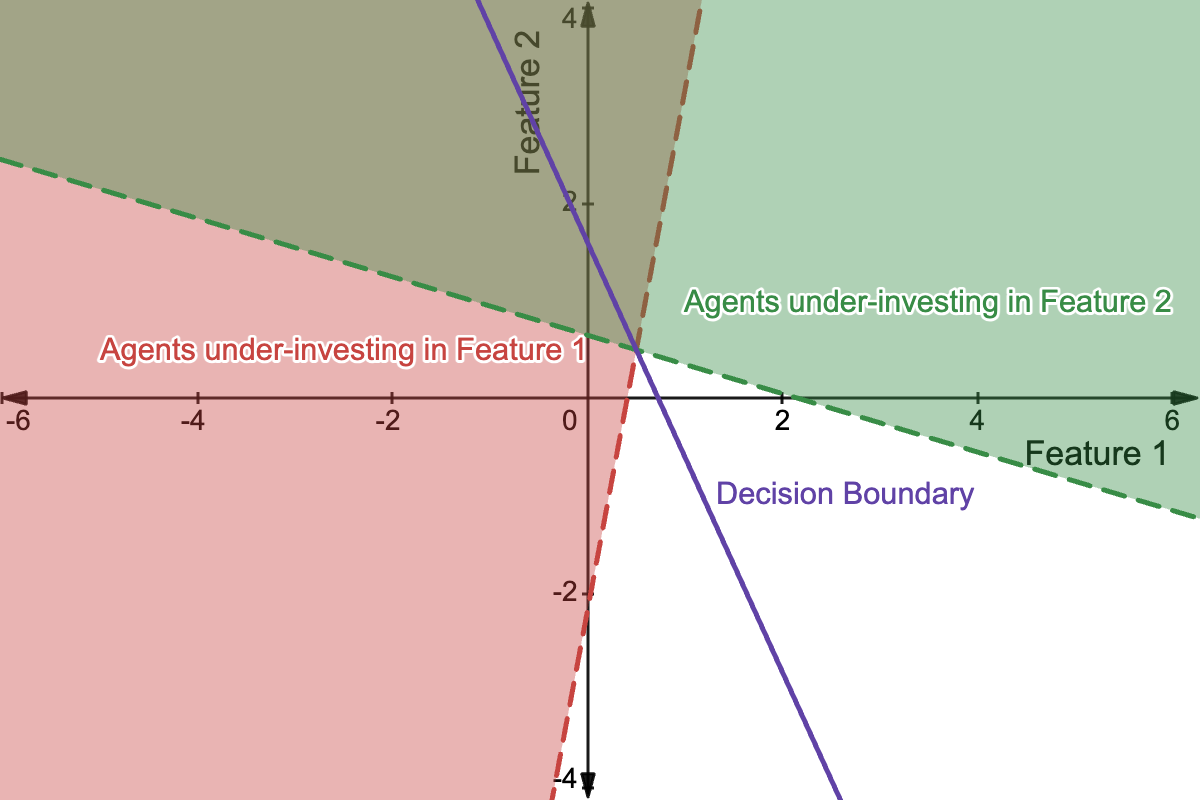
\includegraphics[width=0.5\linewidth]{Figures/desmos-graph.png}
    \caption{Caption}
    \label{fig:unde-over-invest}
\end{figure}
\end{itemize}
For instance, for $\gamma = 0.5$, $\norm{\vtheta}_2=\norm{\vw(\vtheta)}_2$ occurs when $w(\theta) = 0.5425$ and $\theta = 0.6880$ for $w(\theta)<\theta$. Therefore, for $\theta_0 = 0.5$, \eqref{eq:example_underinvest_1} and \eqref{eq:example_underinvest_2} will divide the feature space as in Figure~\ref{fig:unde-over-invest}. 
 
As seen in Figure~\ref{fig:unde-over-invest}, agents with high Feature 2 and low Feature 1 will under-invest in Feature 1 and 2. These agents will not make it to the decision boundary because of under-investment. On the other hand, the agents in the white space of Figure~\ref{fig:unde-over-invest} will over-invest in both features and pass the decision boundary. Their utility will be lower than the non-biased case since they have a higher cost due to aiming for a perceived decision boundary, but they will pass it. 
 
Compared to the non-strategic case, the firm will suffer additional loss only because of agents that over-invest. Therefore, the firm only needs to minimize the loss for agents that manipulate their features and over-invest in both features. It is necessary to note that the discussion above only tells us which agents will under-invest or over-invest in either feature and does not tell us which agents will or will not qualify. For the budgeted problem, the statements remain valid. However, not all the agents will manipulate their features, and only a subset of agents will. 

